\subsection{\texorpdfstring{SYSTEMS OF TYPE \(B_{l}\) (\(l \geqslant 2\))}{SYSTEMS OF TYPE B\_l (l >= 2)}}

\begin{enumerate}
\def\labelenumi{(\Roman{enumi})}
\item
  We consider the group \(L_{0}\) in V = \(R^{l}\) (no. 4). Let R be the set of \(\alpha \in L_{0}\) such that \((\alpha|\alpha) = 1\) or \((\alpha|\alpha) = 2\) , in other words the set of vectors \(\pm\varepsilon_{i}\) ( \(1 \leqslant i \leqslant l\) ) and \(\pm\varepsilon_{i} \pm \varepsilon_{j}\) ( \(1 \leqslant i < j \leqslant l\) ). It is clear that R generates V and that \(2(\alpha|\beta)/(\alpha|\alpha) \in \mathbf{Z}\) for all \(\alpha, \beta \in R\) . Thus R is a reduced root system in V (no. 4). The number of roots is \(n = 2l + 4\frac{l(l-1)}{2} = 2l^{2}\) .
\item
  Put
\end{enumerate}

\[
\alpha_ {1} = \varepsilon_ {1} - \varepsilon_ {2}, \alpha_ {2} = \varepsilon_ {2} - \varepsilon_ {3}, \dots , \alpha_ {l - 1} = \varepsilon_ {l - 1} - \varepsilon_ {l}, \alpha_ {l} = \varepsilon_ {l}.
\]

Then

\[
\begin{array}{c} \varepsilon_ {i} = \alpha_ {i} + \alpha_ {i + 1} + \dots + \alpha_ {l} \quad (1 \leqslant i \leqslant l) \\ \varepsilon_ {i} + \varepsilon_ {j} = (\alpha_ {i} + \alpha_ {i + 1} + \dots + \alpha_ {l}) + (\alpha_ {j} + \alpha_ {j + 1} + \dots + \alpha_ {l}) (1 \leqslant i <   j \leqslant l) \\ \varepsilon_ {i} - \varepsilon_ {j} = \alpha_ {i} + \alpha_ {i + 1} + \dots + \alpha_ {j - 1} \quad (1 \leqslant i <   j \leqslant l). \end{array}
\]

Thus \((\alpha_{1},\alpha_{2},\ldots ,\alpha_{l})\) is a basis of R (§ 1, no. 7. Cor. 3 of Prop. 20). Moreover, \(\| \alpha_{i}\|^{2} = 2\) for \(i < l\) , \(\| \alpha_l\| ^2 = 1\) , \((\alpha_i|\alpha_{i + 1}) = -1\) for \(1\leqslant i\leqslant l - 1\) , \((\alpha_i|\alpha_j) = 0\) for \(j > i + 1\) : the Dynkin graph of R is thus of type \(\mathbf{B}_l\) , which shows that R is irreducible. The positive roots are the \(\varepsilon_{i}\) and the \(\varepsilon_{i}\pm \varepsilon_{j}\) ( \(i < j\) ).

\begin{enumerate}
\def\labelenumi{(\Roman{enumi})}
\setcounter{enumi}{2}
\tightlist
\item
  By Th. 1 (ii) of Chap. V, § 6, no. 2.
\end{enumerate}

\[
h = n / l = 2 l.
\]

\begin{enumerate}
\def\labelenumi{(\Roman{enumi})}
\setcounter{enumi}{3}
\tightlist
\item
  Let \(\tilde{\alpha} = \varepsilon_{1} + \varepsilon_{2} = \alpha_{1} + 2\alpha_{2} + 2\alpha_{3} + \cdots + 2\alpha_{l}\) , which is a root. The sum of its coordinates relative to the basis \((\alpha_{i})\) is 2l - 1 = h - 1. In view of Prop. 31 of § 1, no. 11, \(\tilde{\alpha}\) is the highest root of R. We have \((\tilde{\alpha}| \alpha_{i}) = 0\) for \(i \neq 2\) and \((\tilde{\alpha}| \alpha_{2}) = 1\) . Since \(\alpha_{2}\) is of length 1 (resp. \(\sqrt{2}\) ) when l = 2 (resp. \(l \geqslant 3\) ), the completed Dynkin graph of R is as follows:
\end{enumerate}

\[
\text { for } l = 2 \quad \alpha_ {2} \alpha_ {1}
\]

\pandocbounded{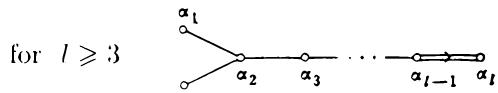
\includegraphics[keepaspectratio]{images/part002_79c781e2.jpg}}

\begin{enumerate}
\def\labelenumi{(\Alph{enumi})}
\setcounter{enumi}{21}
\tightlist
\item
  The formula \(\alpha^{\prime} = \frac{2\alpha}{(\alpha|\alpha)}\) gives for \(R^{\prime}\) the set of vectors \(\pm 2\varepsilon_{i}\) ( \(1 \leqslant i \leqslant l\) ), \(\pm \varepsilon_{i} \pm \varepsilon_{j}\) ( \(1 \leqslant i < j \leqslant l\) ). The Dynkin graph of \(R^{\prime}\) is obtained from that of \(R\) by the procedure explained in no. 2, and we see that \(R^{\prime}\) is of type \(C_{l}\) .
\end{enumerate}

There are \(4l - 2\) roots not orthogonal to \(\beta = \varepsilon_1\) , namely \(\pm \varepsilon_1\) and \(\pm \varepsilon_1 \pm \varepsilon_j\) for \(2 \leqslant j \leqslant l\) ; for each such root \(\alpha\) , \(n(\alpha, \beta) = \pm 2\) . Formula (17) of § 1, no. 12 shows that, for \(\Phi_{\mathrm{R}}\) , the square of the length of \(\beta\) is \((4l - 2)^{-1}\) ; hence \(\Phi_{\mathrm{R}}(x, y) = (x|y)/(4l - 2)\) . Apply formula (18) of § 1, no. 12 with \(x = y = \beta\) . This gives

\[
2 + \frac {1}{4} (4 l - 4) = \gamma (R) \frac {1}{4 l - 2}
\]

and so \(\gamma(R) = (l + 1)(4l - 2)\) .

\begin{enumerate}
\def\labelenumi{(\Roman{enumi})}
\setcounter{enumi}{5}
\tightlist
\item
  The fundamental weights \(\omega_{i}\) ( \(1 \leqslant i \leqslant l\) ) such that \((\omega_{i}|\alpha_{j}) = \delta_{ij}\) are easily calculated, and we find that
\end{enumerate}

\[
\begin{array}{l} \omega_ {i} = \varepsilon_ {1} + \varepsilon_ {2} + \dots + \varepsilon_ {i} \\ \qquad = \alpha_ {1} + 2 \alpha_ {2} + \dots + (i - 1) \alpha_ {i - 1} + i (\alpha_ {1} + \alpha_ {i + 1} + \dots + \alpha_ {l}) (i <   l) \\ \omega_ {l} = \frac {1}{2} (\varepsilon_ {1} + \varepsilon_ {2} + \dots + \varepsilon_ {l}) = \frac {1}{2} (\alpha_ {1} + 2 \alpha_ {2} + \dots + l \alpha_ {l}). \end{array}
\]

\begin{enumerate}
\def\labelenumi{(\Roman{enumi})}
\setcounter{enumi}{6}
\tightlist
\item
  The sum of the positive roots is
\end{enumerate}

\[
\begin{array}{l} 2 \rho = (2 l - 1) \varepsilon_ {1} + (2 l - 3) \varepsilon_ {2} + \dots + 3 \varepsilon_ {l - 1} + \varepsilon_ {l} \\ = (2 l - 1) \alpha_ {1} + 2 (2 l - 2) \alpha_ {2} + \dots + i (2 l - i) \alpha_ {i} + \dots + l ^ {2} \alpha_ {l}. \end{array}
\]

\begin{enumerate}
\def\labelenumi{(\Roman{enumi})}
\setcounter{enumi}{7}
\item
  We have \(Q(R) = L_{0}\) (no. 4), and \(P(R)\) is generated by \(Q(R)\) and \(\omega_{l}\) , hence is equal to \(L_{2}\) (no. 4). Hence, \(P(R)/Q(R)\) is isomorphic to Z/2Z, and the connection index is equal to 2.
\item
  and (X) In \(R^{l}\) , the orthogonal reflection \(s_{\varepsilon_{i}-\varepsilon_{j}}\) ( \(i \neq j\) ) interchanges \(\varepsilon_{i}\) and \(\varepsilon_{j}\) and leaves \(\varepsilon_{k}\) invariant when the index k is distinct from i and j. The \(s_{\varepsilon_{i}-\varepsilon_{j}}\) generate a group \(G_{1}\) isomorphic to the symmetric group \(S_{l}\) . The orthogonal reflection \(s_{\varepsilon_{i}}\) transforms \(\varepsilon_{i}\) to \(-\varepsilon_{i}\) and leaves invariant the \(\varepsilon_{k}\) when the index k is distinct from i. The \(s_{\varepsilon_{i}}\) generate a group \(G_{2}\) isomorphic to \((\mathbf{Z}/2\mathbf{Z})^{l}\) . The Weyl group W(R) is generated by \(G_{1}\) and \(G_{2}\) , and \(G_{2}\) is normal in W(R), so W(R) is isomorphic to the semi-direct product of \(S_{l}\) by \((\mathbf{Z}/2\mathbf{Z})^{l}\) . Its order is therefore \(2^{l}\cdot l!\) .
\end{enumerate}

The symmetric algebra \(\mathbf{S}(\mathbf{R}^{l})\) can be identified canonically with the algebra of polynomial functions \(\mathrm{P}(\xi_{1},\ldots,\xi_{l})\) on \(R^{l}\) . For such a polynomial to be invariant under \(\mathrm{W}(\mathrm{R})\) , it is first of all necessary that

\[
P \left(\xi_ {1}. \xi_ {2}. \dots ., \xi_ {l}\right) = P \left(\pm \xi_ {1}. \pm \xi_ {2}. \dots ., \pm \xi_ {l}\right)
\]

for all choices of the signs on the right-hand side, so that

\[
\mathrm{P} \left(\xi_ {1}, \dots , \xi_ {l}\right) = \mathrm{Q} \left(\xi_ {1} ^ {2}, \dots , \xi_ {l} ^ {2}\right)
\]

where Q is a polynomial, and further that Q is a symmetric polynomial; and these conditions are sufficient. Consequently (Algebra. Chap. V, App. I), \(\mathbf{S}(\mathbf{R}^{l})^{\mathrm{W}(\mathbb{R})}\) is the algebra generated by the l polynomial functions

\[
t _ {i} = \sum_ {\tau \in \mathfrak {S} _ {l}} \xi_ {\tau (1)} ^ {2} \xi_ {\tau (2)} ^ {2} \dots \xi_ {\tau (l)} ^ {2} \quad (1 \leqslant i \leqslant l).
\]

Moreover, the transcendence degree over \(\mathbf{R}\) of the field of fractions of \(\mathbf{S}(\mathbf{R}^l)^{\mathrm{W(R)}}\) is \(l\) , so the \(t_i\) are algebraically independent. Since the \(t_i\) have degree \(2,4,\ldots ,2l\) , we conclude that the exponents of \(\mathrm{W(R)}\) (Chap. V. § 6, no. 3, Prop. 3) are:

\[
1, 3, 5, \dots , 2 l - 1.
\]

\begin{enumerate}
\def\labelenumi{(\Roman{enumi})}
\setcounter{enumi}{10}
\item
  The only automorphism of the Dynkin graph is the identity element. Thus, \(A(R) = W(R)\) and \(-1 \in W(R)\) . Since -1 transforms B to -B, we conclude that \(w_{0} = -1\) .
\item
  The group \(P(R^{\prime})/Q(R^{\prime})\) is dual to \(P(R)/Q(R)\) , and hence is isomorphic to Z/2Z. Its non-trivial element permutes the vertices corresponding to \(\alpha_{0}\) and \(\alpha_{1}\) and leaves the others fixed.
\end{enumerate}
% semantic-fragments: legacy-input-seam
\relax{}
